%*****************************************
\chapter{Preliminaries}\label{ch:Preliminaries}
%*****************************************
%\setcounter{figure}{10}
% \NoCaseChange{Homo Sapiens}

\section{Lloyd-Hoare Logic}
\todo{A history lesson, rewrite to include LLoyd. See \cite{kaminski19} P.27. }

In 1969, C.A.R. Hoare wrote \textit{An Axiomatic Basis for Computer Programming}~\cite{hoare69} to explore the logic of computer programs use axioms and inference rules to prove the properties of programs. 
This system is known as \define{Hoare Logic}. 
He introduced \imptt{sufficient} preconditions that will guarantee correct results but does not rule out non-termination. 
A selection of the axioms and rules are shown in \autoref{tab:hoare}. \footnote{We omit the symbol $\vdash$ in front of a Hoare Triple, which denotes ``valid/provable'', for better readability. }\footnote{Non-determinism was not considered in the original paper, so we treat the programs here as deterministic. 
With deterministic programs, one initial state corresponds to one final state, and by non-termination we assign a final state $\bot$. \todo{Think about whether to add liberally deterministic (Hesselink 1992, Programs, Recursion and Unbounded Choice). }} 


\begin{table}[ht]\centering
    \begin{tabular}{ll}
      \hline \hline
      \textbf{Axiom of Assignment}     &  \hoare{F[x/e]}{x:=e}{F}   \\
      \textbf{Rules of Consequence}   &  If \hoare{G}{C}{F} and $F\Rightarrow P$ then \hoare{G}{C}{P} \\
                                      &  If \hoare{G}{C}{F} and $P\Rightarrow G$ then \hoare{P}{C}{F} \\
      \textbf{Rule of Composition}   &  If \hoare{G}{C_1}{F_1} and \hoare{F_1}{C_2}{F} then \hoare{G}{C_1;C_2}{F} \\
      \textbf{Rule of Iteration}  &  If $F\wedge$(\hoare{B}{C}{F}) then \hoare{F}{\text{while } B \text{ do } C }{\neg B \wedge F}  \\
      % \textbf{Rule of Condition}   &  $wp.C_1.(wp.C_2.F)$\\
      \hline\hline
    \end{tabular}
    \caption{Valid Hoare Triples}
    \label{tab:hoare}
\end{table}

\mathl{\{F[x/e]\}} is obtained by substituting occurrences of $x$ by $e$. 

Semantically, a Hoare Triple {{\color{Gray}{\hoare{G}{C}{F}}}} is said to be valid for (partial) correctness, if the execution of the program $C$ with an initial state satisfying the precondition $G$ leads to a final state that satisfies the postcondition $F$, provided that the program terminates. 

The definition indeed corresponds to this intended semantics. (Formal soundness proofs can be found in Krzysztof R. Apt's survey~\cite{apt81} in 1981. )
As an example, consider the rule of composition: if the execution of program $C_1$ changes the state from $G$ to $F_1$, and $C_2$ changes the state from $F_1$ to $F$, then executing them consecutively should bring the program state from $G$ to $F$, with the intermediate state $F_1$.

The missing guarantee of termination can be seen in the rule of iteration: consider the example 
\todo{Add example here. }

\autoref{fig:hoare} illustrates a valid Hoare Triple, $\Sigma$ represents the set of all states, the section denoted with $G$ includes the states that satisfy the predicate $G$. The arrow from left to write denotes the execution of the program $C$. 

\todo{In case I change color for $\backslash$ mathl, I should change the color for hoare triplc GCF. }

\begin{figure}[ht!]\centering
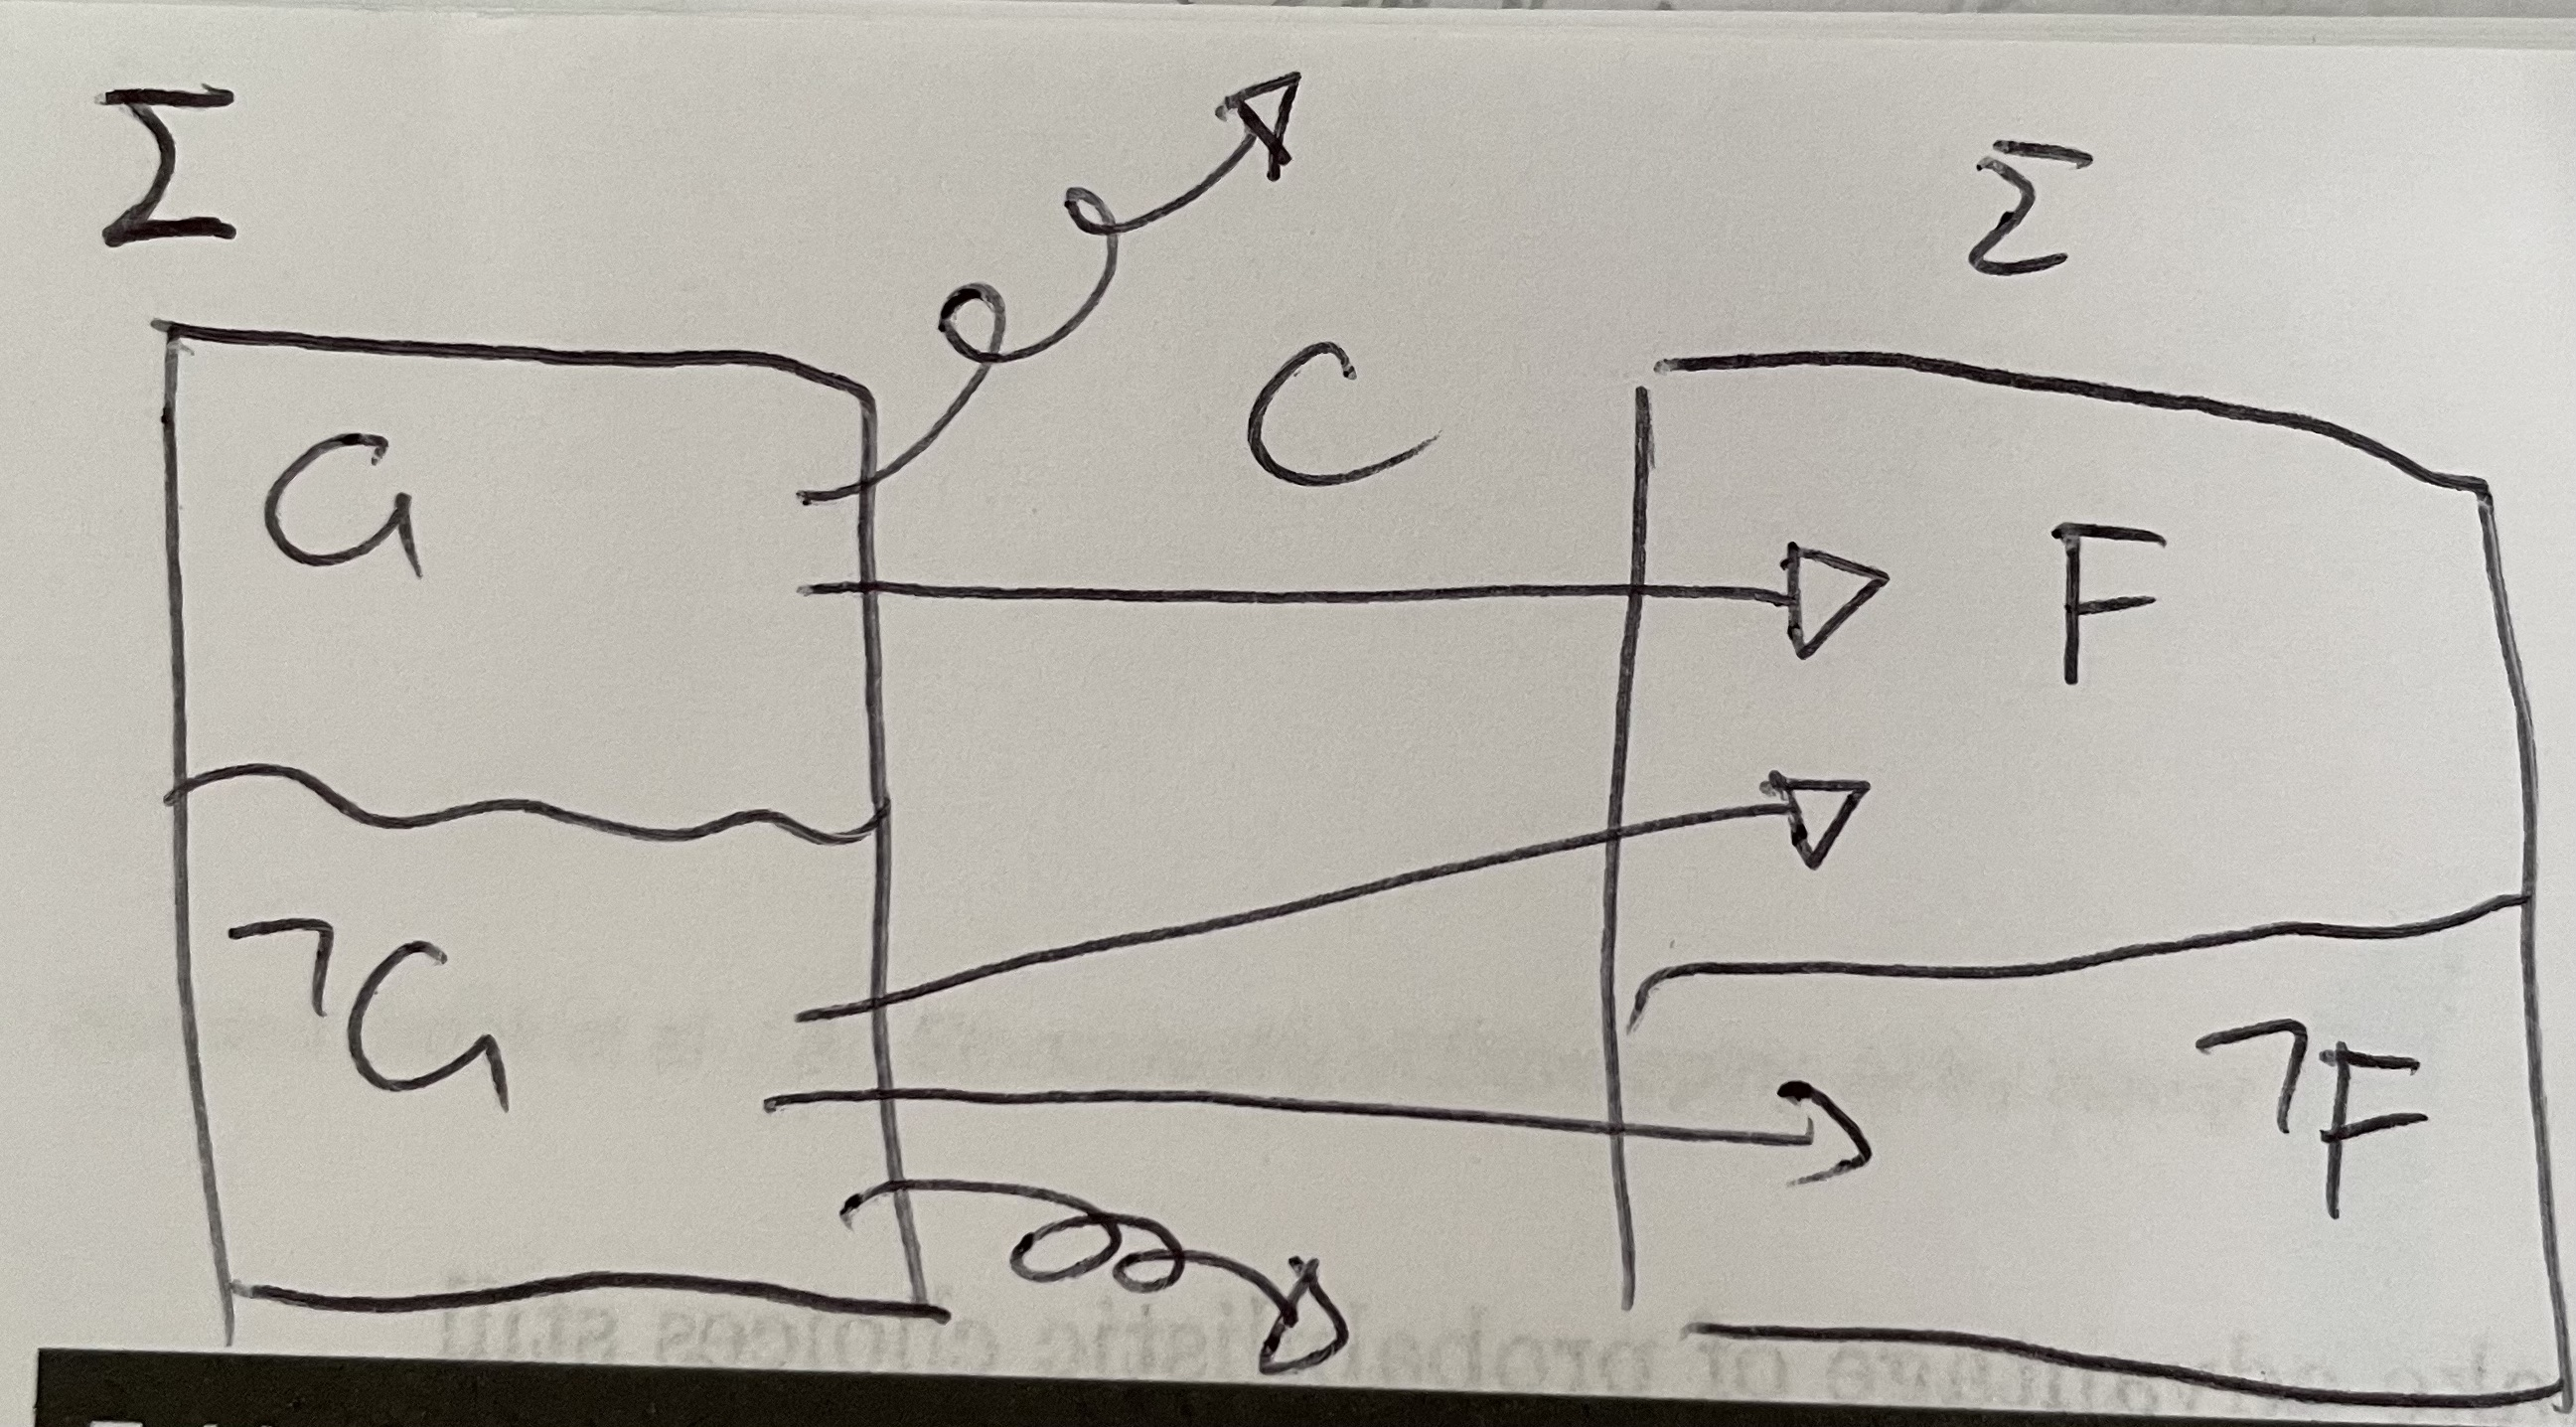
\includegraphics[width=0.5\textwidth]{image/hoare.jpg}
\caption{Valid Hoare Triple (Deterministic)}
\label{fig:hoare}
\todo{Digitize image. }
\end{figure}


Hoare Logic is sound, expressive, yet incomplete~\cite{apt81}.
A sensible advancement would be to find the \imptt{necessary and sufficient} preconditions that grant us the post-properties, i.e. to eliminate the arrows from $\neg G$ to $F$ in \autoref{fig:hoare}, and to be able to prove termination, i.e. to eliminate the arrows from $G$ to the abyss\footnote{Adding termination proof is also done by Zohar Manna and Amir Pnueli in 1974~\cite{manna74}, where they introduced what we call a \define{loop variant}, a value that decreases with each iteration. The name is in contrast to \define{loop invariant}, concretely the $F$ in Rule of Iteration, which is constant before and after the loop. }, which is what Edsger W Dijkstra accomplished with his \define{weakest precondition} transformer in 1975~\cite{dijkstra75}, among other things. 


\section{Guarded Command Language}\label{sec:gcl}
From now on we will use Dijkstra's (non-deterministic) \define{guarded command language (GCL)}~\cite{dijkstra75} to represent programs and to include non-determinism (starting from \autoref{sec:wp-nondet}).
For better understanding, we use an equivalent
\footnote{Specifically, \mathl{if\ (\varphi)\ \{C_1\}\ else\ \{C_2\}}  is equivalent to
\mathl{if\ \varphi \to C_1\ []\ \neg\varphi \to C_2\ fi} in Dijkstra's original style\cite{dijkstra75}; \mathl{\{C_1\}\square \{C_2\}} is equivalent to \mathl{if\ true\to C_1\ []\ true\to C_2\ fi}.} 
form of GCL that is similar to modern pseudo-code:

\begin{table}[ht!]\centering
    \begin{tabular}{cl}
    $C\ ::=$ &  $x:= e   \ \ \mid \ \  C;C  \ \ \mid \ \   \{C\}\square \{C\}  \ \ \mid \ \  if\ (\varphi)\ \{C\}\ else\ \{C\} 
     \ \ \mid\ \  while\ (\varphi)\ \{C\}$ \\ 
  &$\mid skip \mid diverge$
    \end{tabular}
\end{table}

The \define{non-deterministic choice} \mathl{\{C_1\}\square \{C_2\}} chooses from two programs randomly. 
It is however not \define{probabilistic}, where we know the probabilistic distribution of the outcome of the choice. 
With the non-deterministic choice, we have no such knowledge. 

When \mathl{skip} is executed, the program state does not change and the consecutive part is executed. 
When \mathl{diverge} is executed, the program goes to state $\bot$ to denote non-termination, and the execution stops. 


\section{Weakest Precondition}\label{sec:wp}

\subsection{The Deterministic Case}\label{sec:wp-det}
To better relate Hoare Triples and Dijkstra's weakest precondition transformer, we first ignore non-determinism. 

Again, the goal is to find the \imptt{necessary and sufficient} precondition such that the program is guaranteed to \imptt{terminate} in a state that satisfies the postcondition. 
\autoref{fig:wp-det} shows it graphically. 

\begin{figure}[ht!]\centering
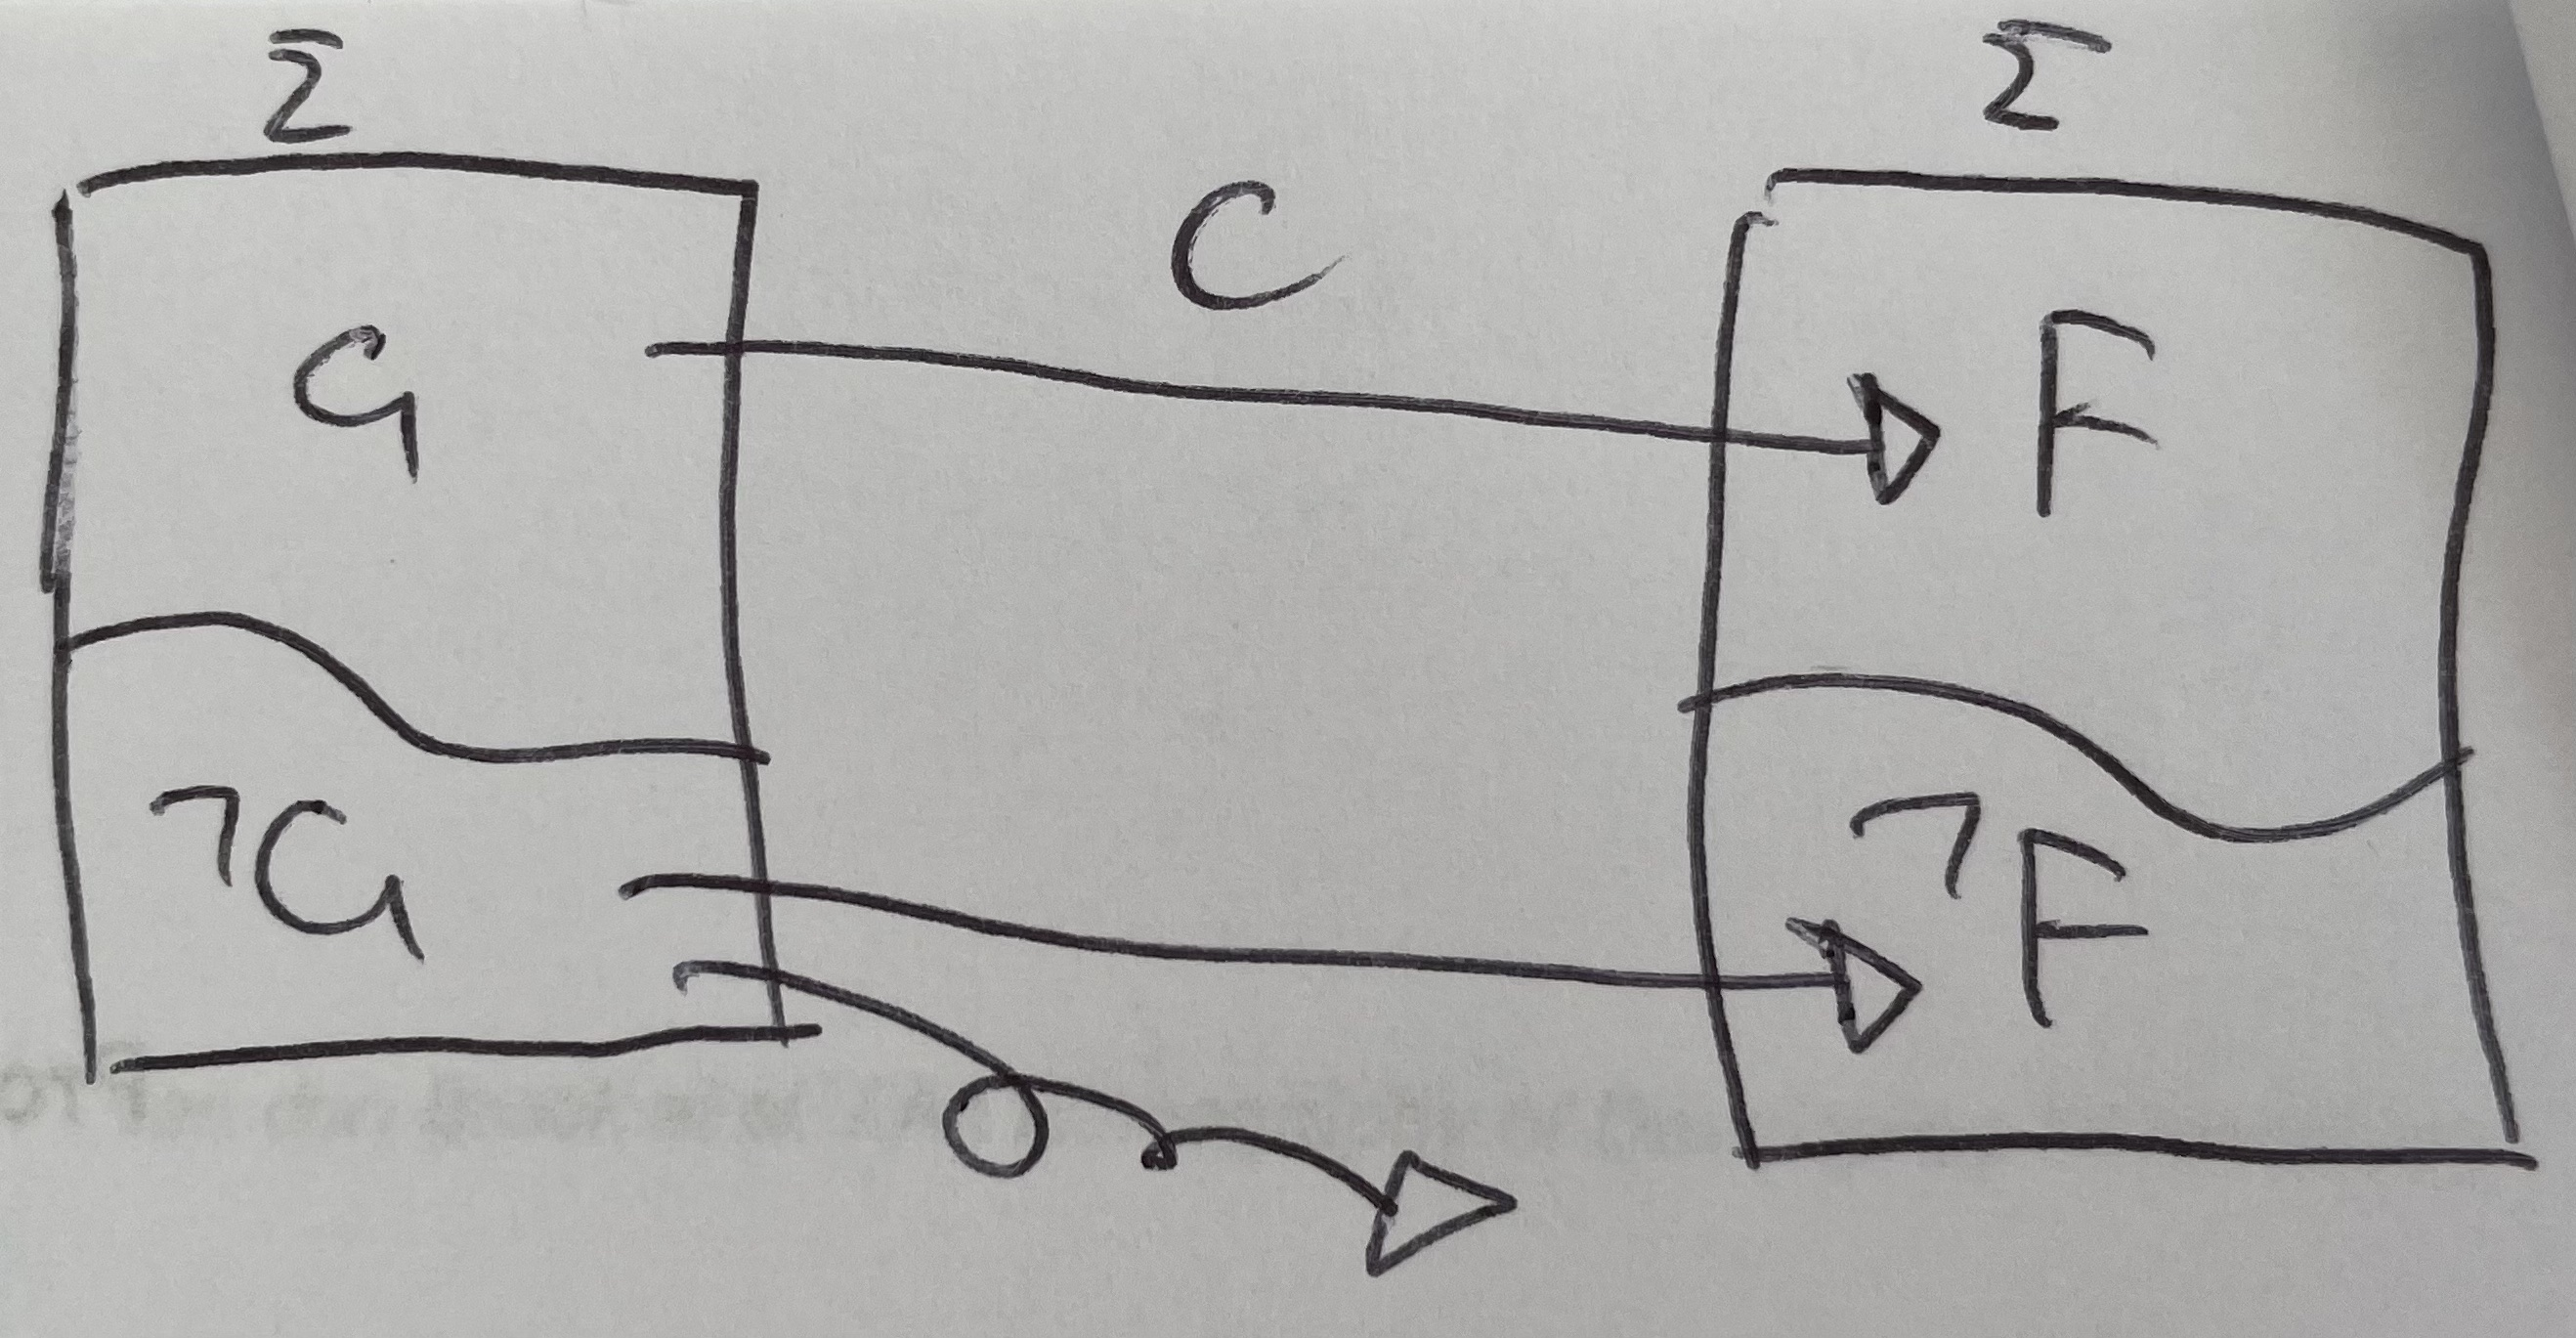
\includegraphics[width=0.5\textwidth]{image/wp-det.jpg}
\caption{Weakest Precondition (Deterministic)}
\label{fig:wp-det}
\todo{Digitize image. }
\end{figure}

We define the \define{weakest precondition} transformer structurally in lambda-calculus style\footnote{For example, $wp.C.F$ can be seen as $wp(C,F)$ in ``typical'' style, where $wp$ is treated as a function that has two parameters. The advantage of lambda-calculus style is scalability, we can simply extend the aforementioned function like $wp.C.F.\sigma$ where $\sigma$ means the initial state. Here $wp$ is treated as a function that has three parameters, if we were to write it in the ``typical'' style. It is then questionable whether we changed the type of $wp$. } as in \autoref{tab:wp-det}: 

\begin{table}[ht!]\centering
    \begin{tabular}{ll}
    \hline\hline
      \textbf{C}&\textbf{wp.C.F}    \\ \hline
      $skip$&   $F$   \\
      $diverge$&  $false$\\
      $x:= e $&  $F[x/e]$\\
      $C_1;C_2$&  $wp.C_1.(wp.C_2.F)$\\
      $if\ (\varphi)\ \{C_1\}\ else\ \{C_2\} $&  $(\varphi\wedge wp.C_1.F)\vee(\neg\varphi\wedge wp.C_2.F)$\\
      % $\{C_1\}\square \{C_2\}$ & $wp.C_1.F\vee wlp.C_2.F$ \\
      $while\ (\varphi)\ \{C'\}$&  $lfp\ X.(\neg\varphi\wedge F)\vee(\varphi\wedge wp.C'.X)$\\
    \hline\hline
    \end{tabular}
    \caption{The Weakest Precondition Transformer (Deterministic Programs)~\cite{kaminski19}}
    \label{tab:wp-det}
\end{table}

\mathl{F[x/e]} is $F$ where every occurrence of $x$ is syntactically replaced by $e$. 

\mathl{lfp\ X. f} is the least fixed point of function $f$ with variable $X$. 

Let {$$\Phi(X):=(\neg\varphi\wedge F)\vee(\varphi\wedge wp.C'.X)$$} be the characteristic function, then $wp$ for while-loop can be defined as: 
{$$wp.(while(\varphi)\{C'\}).F = lfp\ X. \Phi(X)$$}. 

Most of the definitions in \autoref{tab:wp-det} are intuitive and correspond to their counterparts in Hoare Logic.
To take special notice are the definitions for \mathl{diverge} and \mathl{while}. 
Since $wp$ aims for total correctness, the precondition \mathl{wp.diverge.F} should terminate with postcondition \mathl{F}. 
Because \mathl{diverge} does not terminate, there is no such precondition and $wp$ for \mathl{diverge} should be \mathl{false}. 

The definition for the while-loop\cite{kaminski19} is trickier, but we can verify its correctness by recalling Dijkstra's original definition. 

\todo{Find out if there's earlier definition that used lfp. }

\subsection{Defining Loops}
In Dijkstra's original paper\cite{dijkstra75}, he defined $wp$ for while-loops based on its (intended) semantics, i.e. the precondition such that, when satisfied, guarantees that the loop terminates with the required postcondition within a certain number of iterations. 

Let 
\[
WHILE=while(\varphi)\{C'\}
\\ 
IF=  if\ (\varphi)\{C';WHILE\}\ else\ \{skip\}
\] 
Rewriting Dijkstra's definition in a form conforming to our style, he defines 
\[
H_0(F)=(F \wedge \neg \varphi )
\\
H_k(F)=(wp.IF.(H_{k-1}(F)) \vee H_0(F))
\]
Intuitively, when $H_0(F)$ is satisfied before the execution of $WHILE$, the loop is exited with 0 iteration in a state that satisfies $F\wedge\neg\varphi$ hence $F$. 
Then we can understand $H_k(F)$ as the weakest precondition such that the program terminates in a final state satisfying $F$ after \imptt{at most} $k$ iterations. 

Then by definition: 
\begin{equation}
\hspace{2.8cm} wp.WHILE.F=(\exists k\geq 0: H_k(F))  \label{eq:while}
\end{equation}
% \[wp.WHILE.F=(\exists k\geq 0: H_k(F))  \] \label{eq:while}



We state that our definition coincides with this definition. 
Without going too deep into domain theory, we only use one of its theorem that yields a computation for least fix points, when they exist. 

\begin{theorem}
\todo{Insert theorem, then explain least point iteration from bottom. }
\end{theorem}


Coincidentally, $H_k(F)$ is the $k-$th iteration from bottom $\bot$ to calculate the least fixed point of the characteristic function: $\Phi^k(\bot)$. 
Thus by finding the least fixed point, we've found a $k$ that satisfies \eq{while}. 




\subsection{The Non-deterministic Case}\label{sec:wp-nondet}
Now we bring the non-deterministic choice back into the picture and add its definition as shown in \autoref{tab:wp-nondet}. 

\begin{table}[ht!]\centering
    \begin{tabular}{ll}
    \hline\hline
      \textbf{C}&\textbf{wp.C.F}    \\ \hline
      $skip$&   $F$   \\
      $diverge$&  $false$\\
      $x:= e $&  $F[x/e]$\\
      $C_1;C_2$&  $wp.C_1.(wp.C_2.F)$\\
      $if\ (\varphi)\ \{C_1\}\ else\ \{C_2\} $&  $(\varphi\wedge wp.C_1.F)\vee(\neg\varphi\wedge wp.C_2.F)$\\
      {\color{Maroon}$\{C_1\}\square \{C_2\}$} & {\color{Maroon}$wp.C_1.F\vee wlp.C_2.F$}\\
      $while\ (\varphi)\ \{C'\}$&  $lfp\ X.(\neg\varphi\wedge F)\vee(\varphi\wedge wp.C'.X)$\\
    \hline\hline
    \end{tabular}
    \caption{The Weakest Precondition Transformer (Non-deterministic Programs)~\cite{kaminski19}}
    \label{tab:wp-nondet}
\end{table}

To justify this definition for the non-deterministic choice, we must first clarify the intended semantics/meaning of the wp-transformer. 

Let \mathl{\exec C} denote the \define{execution} of program $C$, \mathl{\exec C.\sigma} denote the set of final states that \imptt{can} occur after the execution of $C$. 

(A state is a function that maps a program variable to a value. The set of \define{states} is denoted by \mathl{\Sigma=\{\sigma \mid \sigma: Vars\to Vals\}}. )

If $C$ is deterministic, then $\exec C.\sigma$ is a set of a single state, either a final state $\sigma'$ or $\bot$, if the execution does not terminate. 
If $C$ is non-deterministic, $\exec C.\sigma$ can be a set with multiple elements, since multiple final states can be possible. 

The weakest precondition $wp.C.F$ is then 

\note{Up to here is readable. }

\autoref{fig:wp-nondet} shows $wp$ with non-deterministic programs. 
Each arrow from left to right shows a \imptt{possible} execution of program $C$. 

\begin{figure}[ht!]\centering
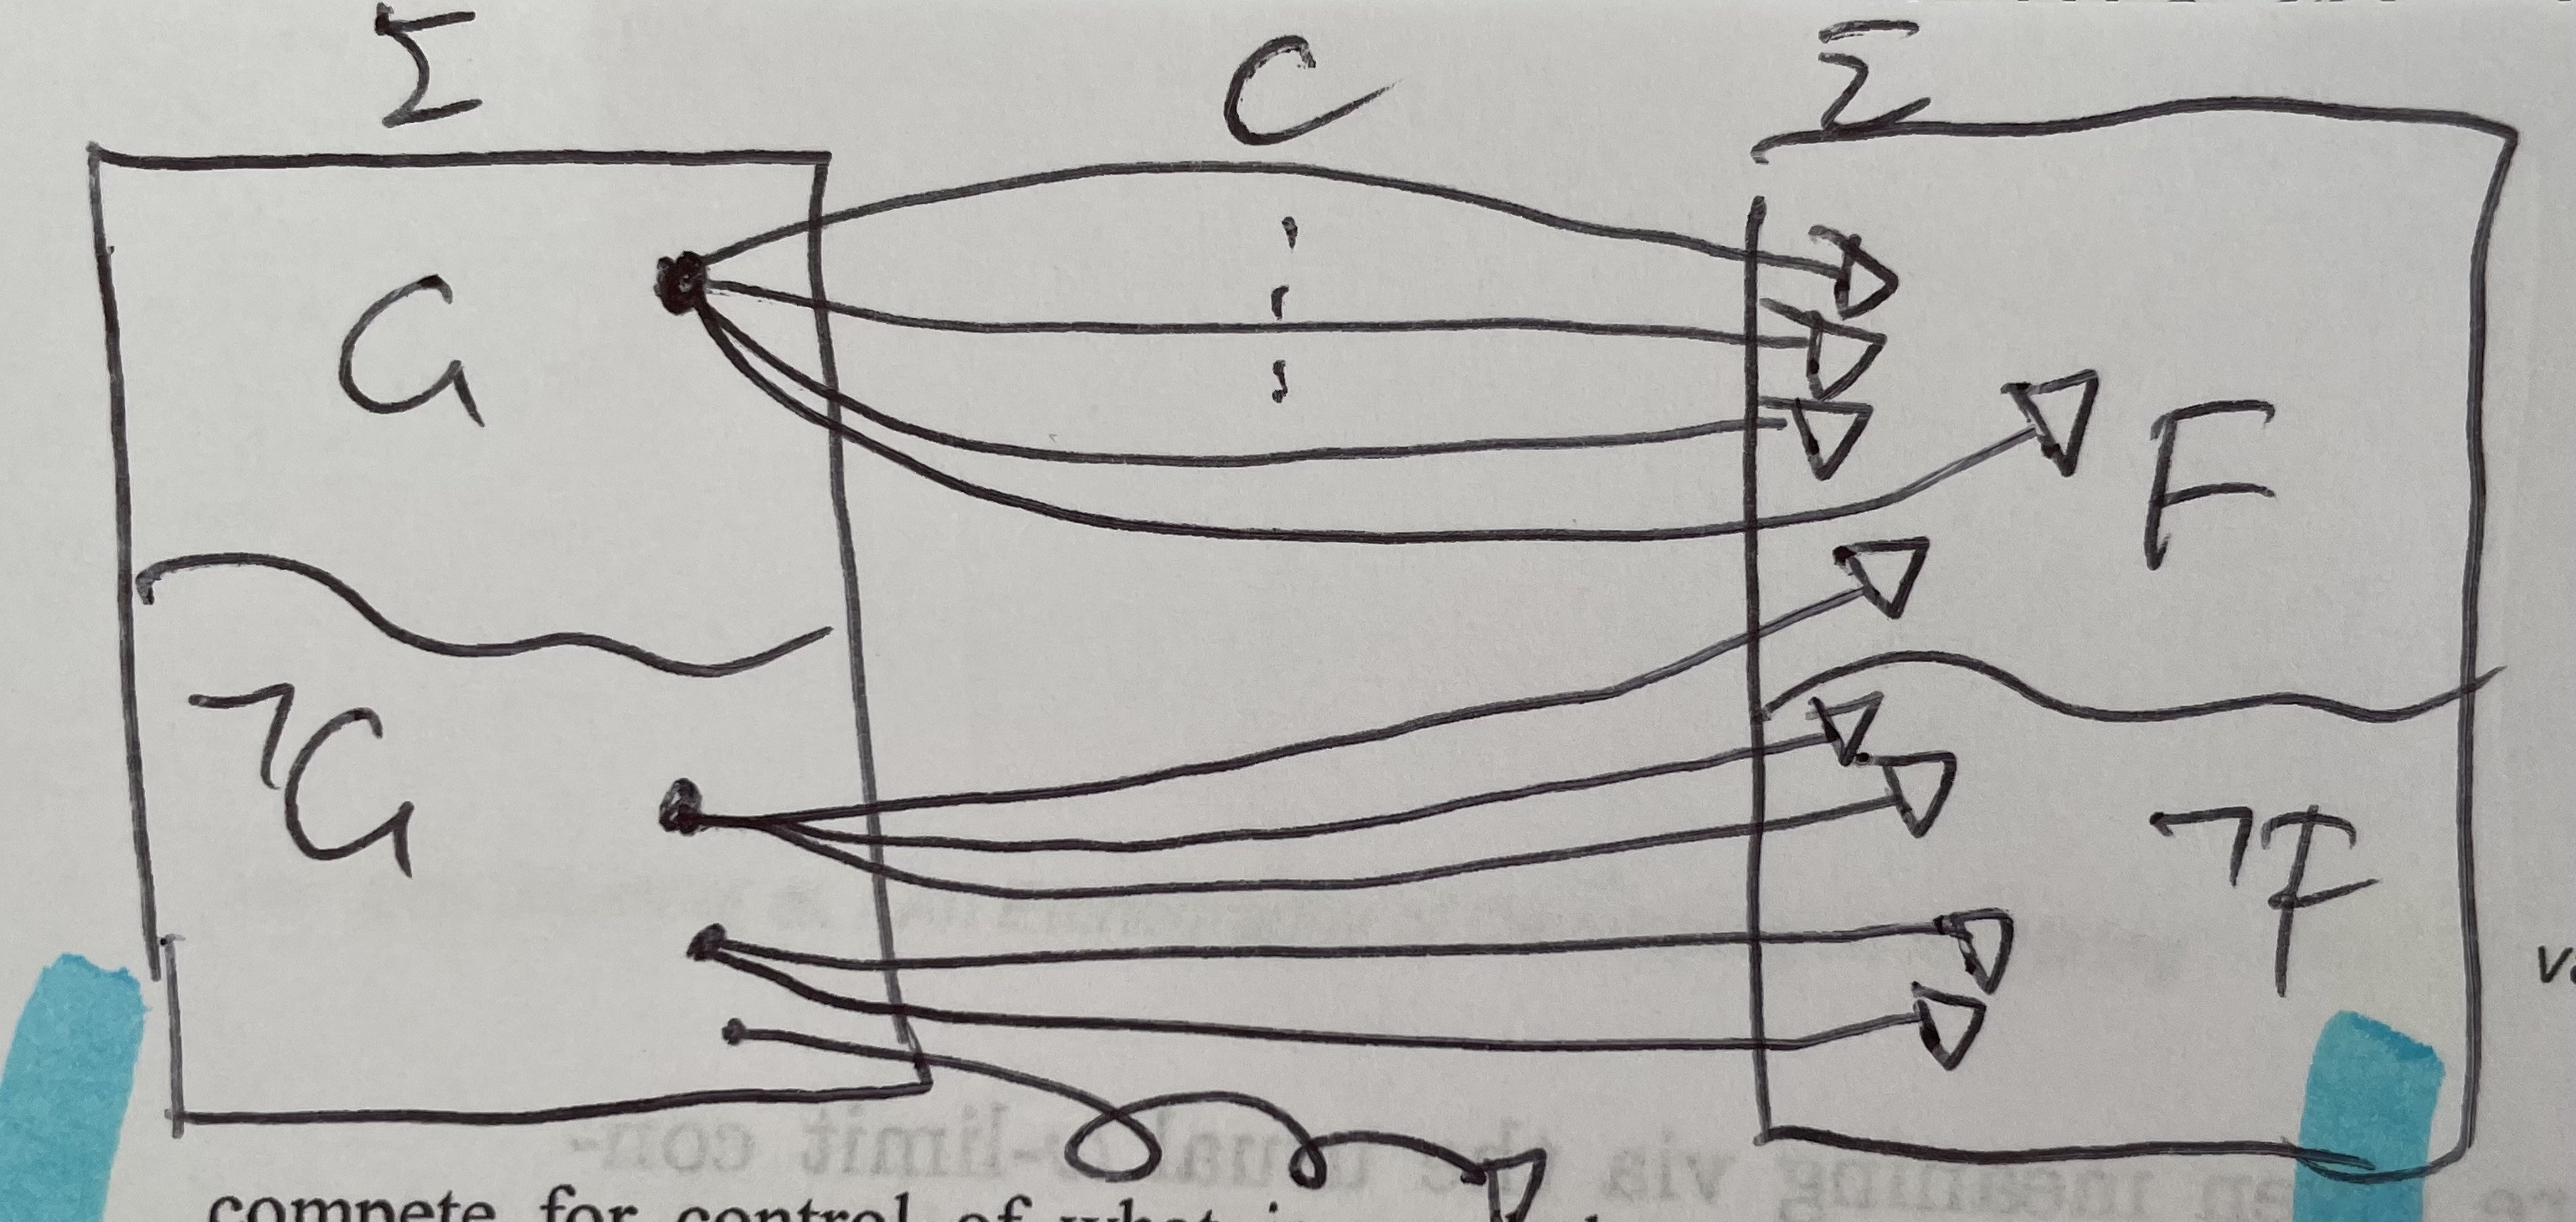
\includegraphics[width=0.5\textwidth]{image/wp-nondet.jpg}
\caption{Weakest Precondition (Non-deterministic)}
\label{fig:wp-nondet}
\todo{Digitize image. }
\end{figure}








\section{Weakest Liberal Precondition}
We define the weakest liberal precondition transformer in \autoref{tab:wlp}. 
\begin{table}[ht!]\centering
    \begin{tabular}{ll}
    \hline\hline
      \textbf{C}&\textbf{wlp.C.F}    \\ \hline
      $skip$&   $F$   \\
      $diverge$&  $true$\\
      $x:= e $&  $F[x/e]$\\
      $C_1;C_2$&  $wp.C_1.(wp.C_2.F)$\\
      $if\ (\varphi)\ \{C_1\}\ else\ \{C_2\} $&  $(\varphi\wedge wp.C_1.F)\vee(\neg\varphi\wedge wp.C_2.F)$\\
      $\{C_1\}\square \{C_2\}$ & $wlp.C_1.F\wedge wlp.C_2.F$\\
      $while\ (\varphi)\ \{C'\}$&  $gfp\ X.(\neg\varphi\wedge F)\vee(\varphi\wedge wp.C'.X)$\\
      \hline\hline
    \end{tabular}
    \caption{The Weakest Liberal Precondition Transformer}
    \label{tab:wlp}
\end{table}

%*****************************************
%*****************************************
%*****************************************
%*****************************************
%*****************************************
